%!TEX program = xelatex
\documentclass[xcolor={table}]{beamer}

\usepackage[brazil]{babel}	
\usepackage[utf8]{inputenc}
\usepackage[T1]{fontenc}
\usepackage[scaled]{helvet}
\usepackage{amsthm}
\usepackage{ragged2e}
\usepackage{subfig}
\usepackage[table]{xcolor}
\usepackage{multicol}
\usepackage{multirow}
\usepackage{fancyvrb}
\usepackage{verbatim}
\usepackage{subcaption}
\usepackage{wrapfig}
\usepackage{lipsum}  
\usepackage{listings}
\usepackage{url}
\usepackage{graphicx}
\usepackage{hyperref}


\usetheme{Execushares}

   \begin{subfigure}
           \hspace*{0.1in}

        \vspace*{0.2in}
           
\includegraphics[scale=0.45]{img/URJC_logo.png}
            \label{fig:urjc}
        \end{subfigure}
        \begin{subfigure}
            
\includegraphics[scale=0.36]{img/betsitLogo.png}
            \label{fig:etsit}
        \end{subfigure}

\vspace{0.8cm}
\title{Mejoras en entorno de robótica  educativa para niños}
\subtitle{Trabajo de fin de grado}
\author[1]{Rubén Álvarez Martín}

\date{Noviembre, 2019}

\begin{document}
	\setcounter{showProgressBar}{0}
	\setcounter{showSlideNumbers}{0}

	\frame{\titlepage}

	\begin{frame}
		\frametitle{Índice}
		\begin{enumerate}
			\item Introducción  \textcolor{ExecusharesGrey}{}
		 \textcolor{ExecusharesGrey}{\footnotesize\hspace{0.5em}}
 		\item Objetivos  \textcolor{ExecusharesGrey}{}
		 \textcolor{ExecusharesGrey}{\footnotesize\hspace{0.5em}}
			\item Herramientas  \textcolor{ExecusharesGrey}{\footnotesize\hspace{0.5em}}
			\item Mejoras a WebSim  \textcolor{ExecusharesGrey}{
			\begin{itemize}
			    \item Soporte a drones en WebSim
			    \item Teleoperadores en WebSim
			    \item Ejercicios individuales
			    \item Ejercicios competitivos
			\end{itemize}} 
			\item Conclusiones  \textcolor{ExecusharesGrey}{\footnotesize\hspace{0.5em}}
		\end{enumerate}
	\end{frame}

	\setcounter{framenumber}{0}
	\setcounter{showProgressBar}{1}
	\setcounter{showSlideNumbers}{1}
	\section{Introducción}
		\begin{frame}
			\frametitle{Tecnologías web}
			\begin{itemize}
			    \item HTTP
			    %imagen http
			    \item Tecnologías en cliente: HTML, CSS y JavaScript. 
			    \item Tecnologías en servidor: Node.js, Django y Spring. 
			\end{itemize}
		\end{frame}
		
		
		\begin{frame}
		\frametitle{Robótica}
        \begin{figure}[H]
        \centering
        \begin{subfigure}{\textwidth}
            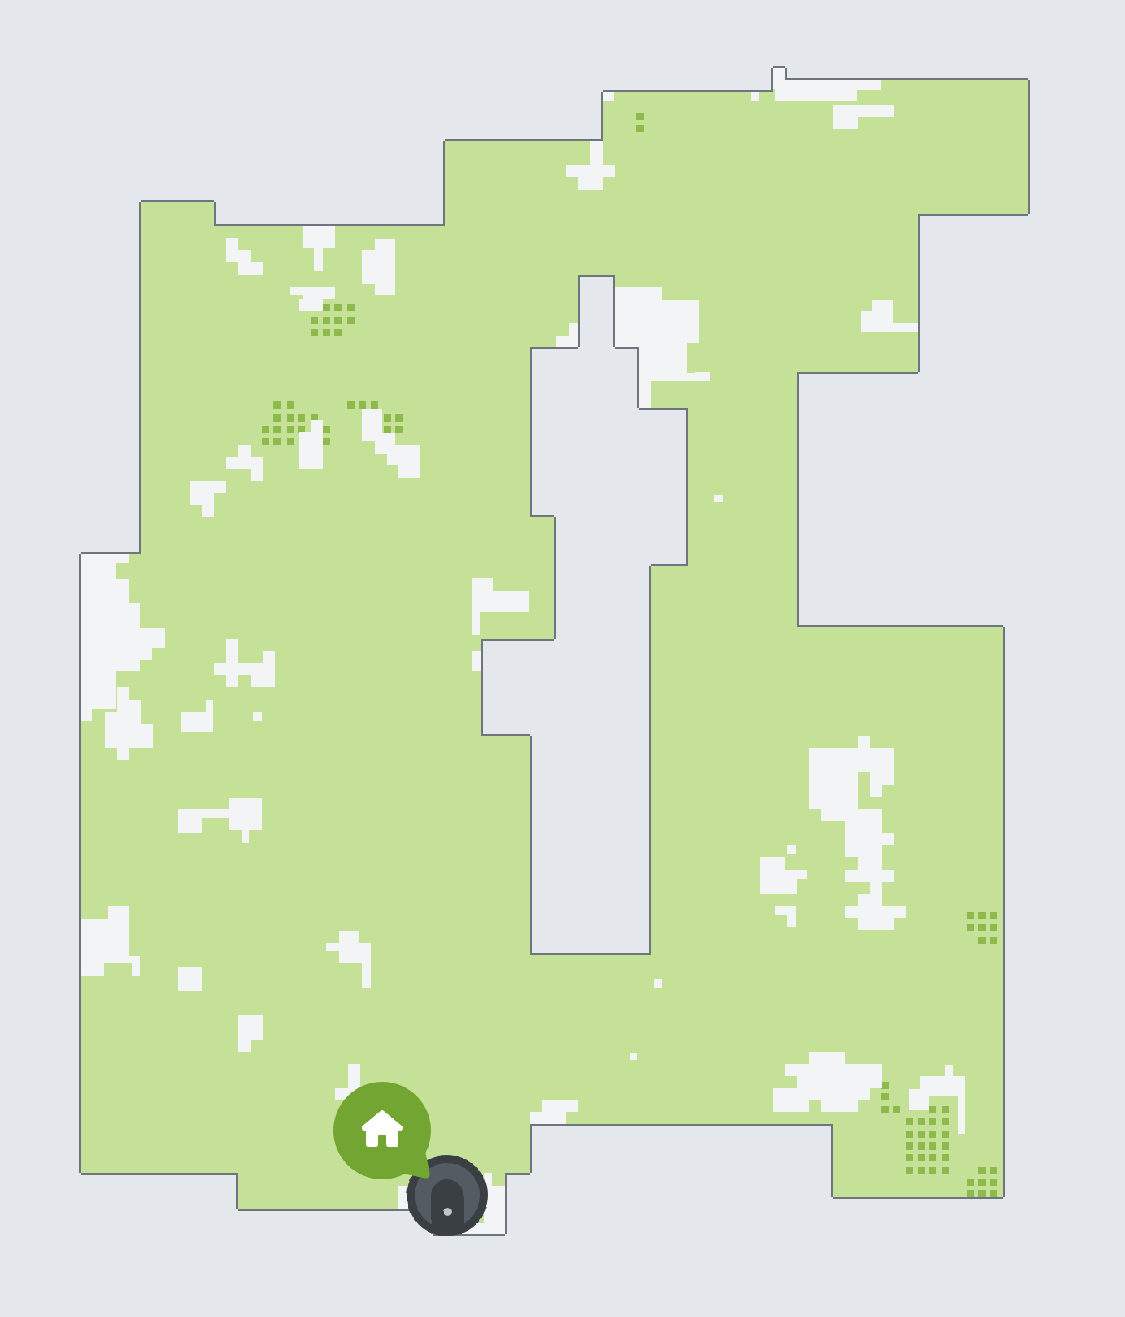
\includegraphics[width=5cm, height=3.5cm]{img/roomba.png}
        \label{fig:roomba}
        \end{subfigure}\hfill
        \begin{subfigure}{\textwidth}
            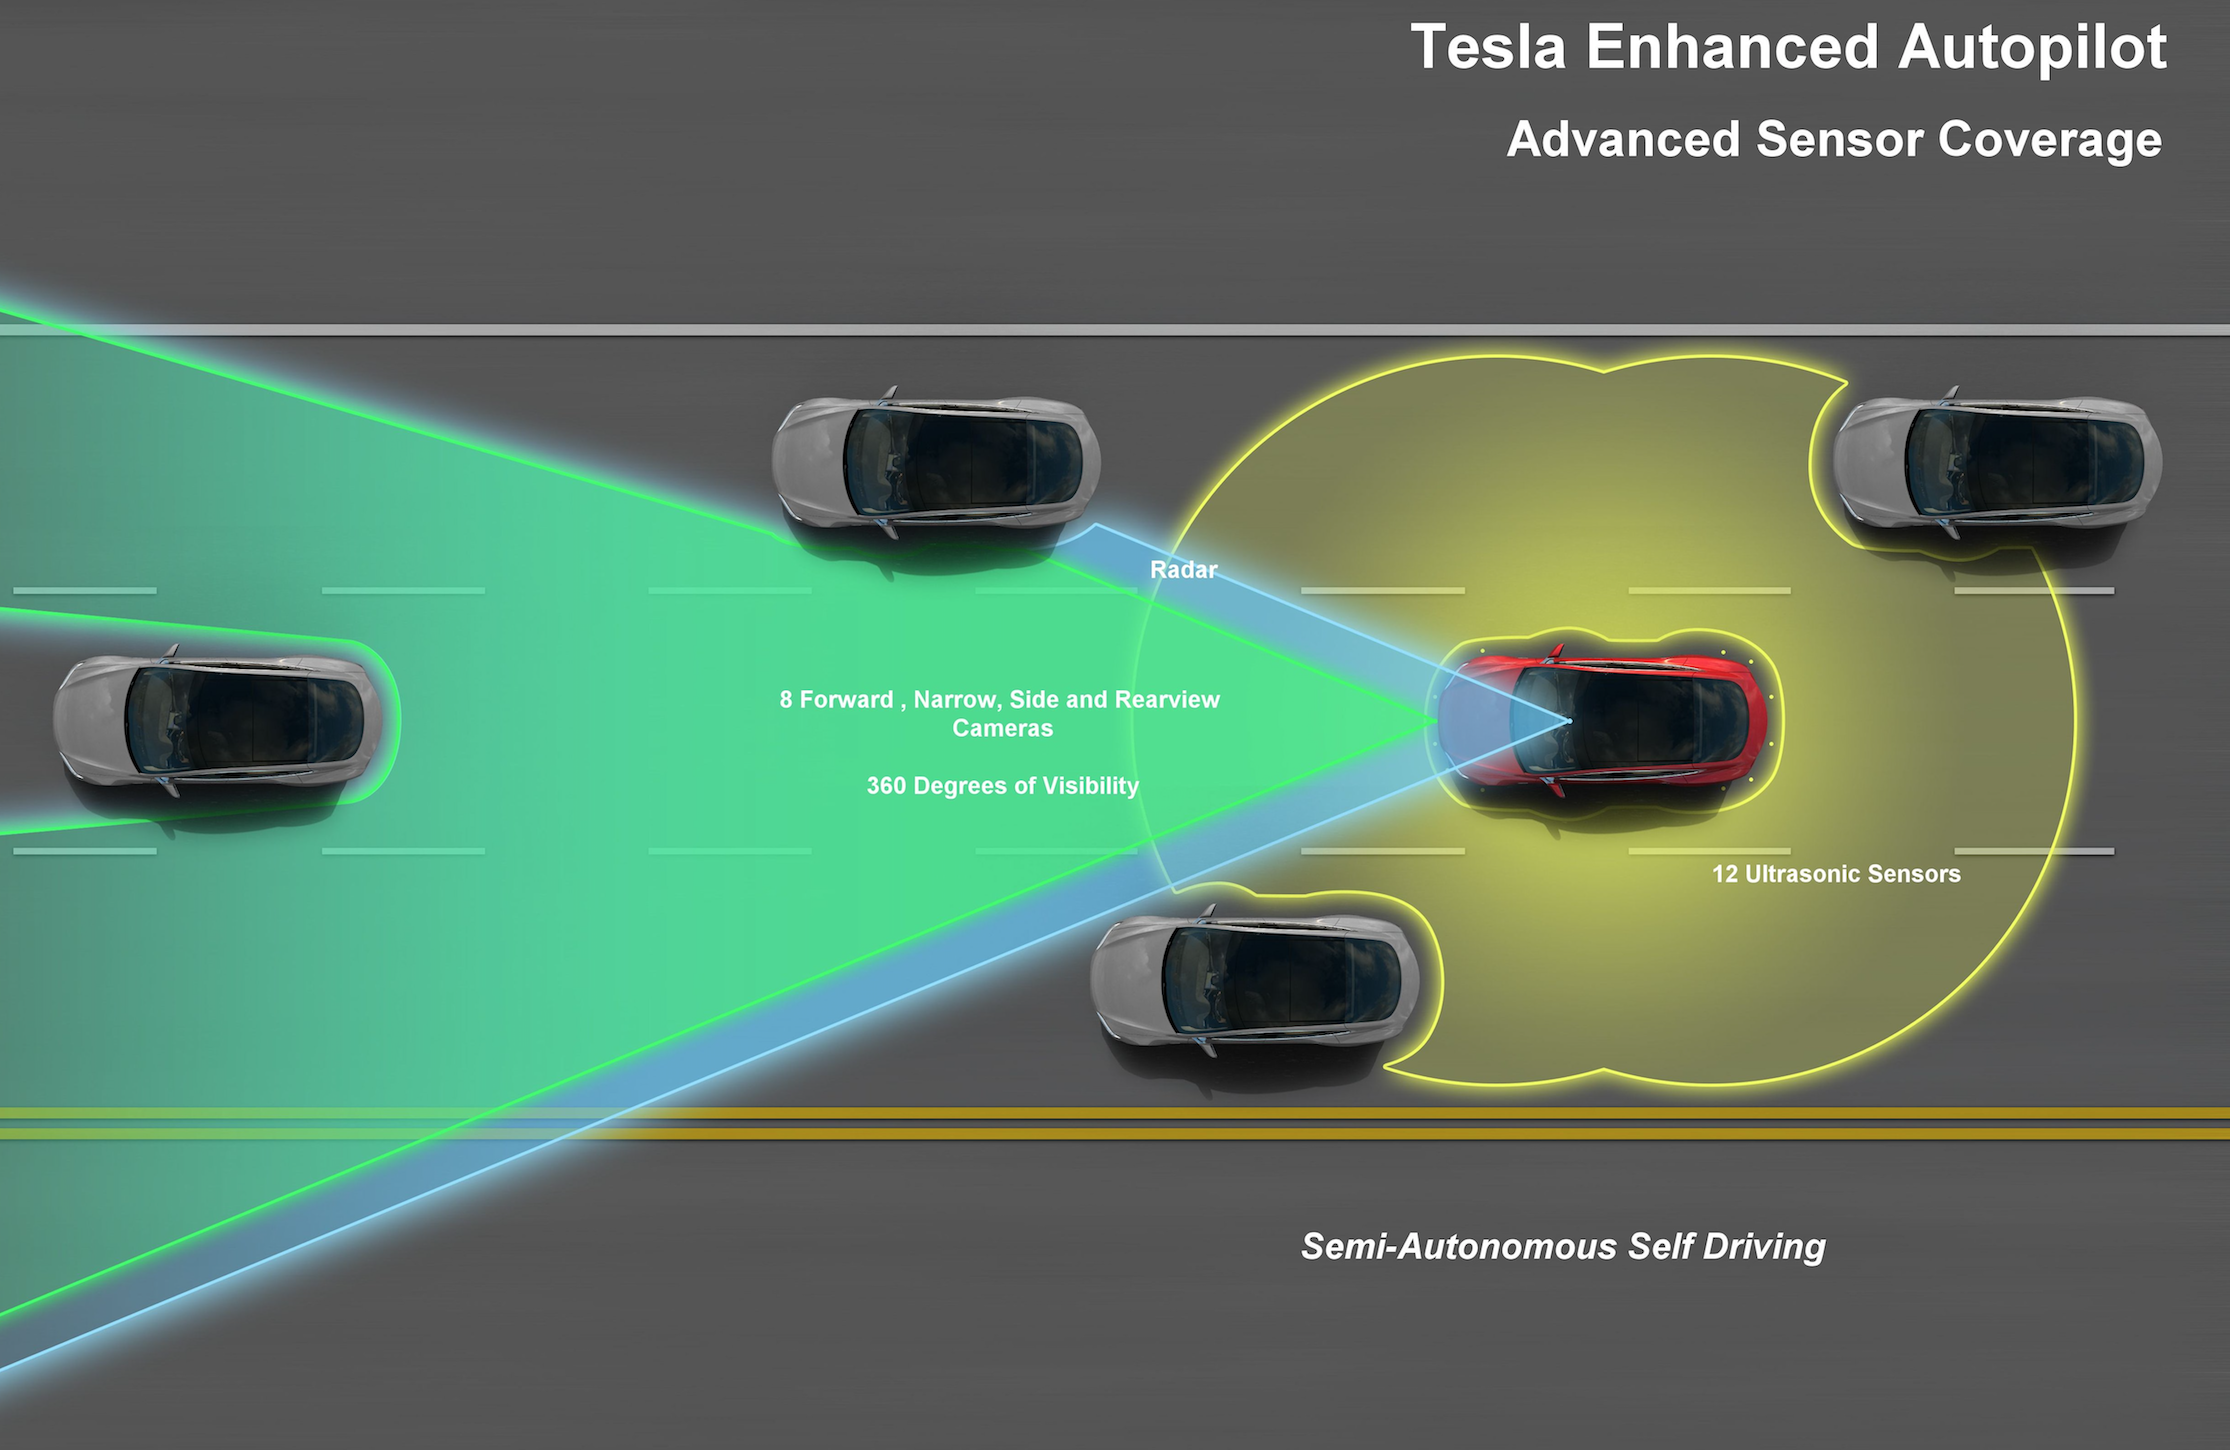
\includegraphics[width=5cm, height=3.5cm]{img/teslaSensors.png}
        \label{fig:tesla}
        \end{subfigure}\hfill
        \begin{subfigure}{\textwidth}
            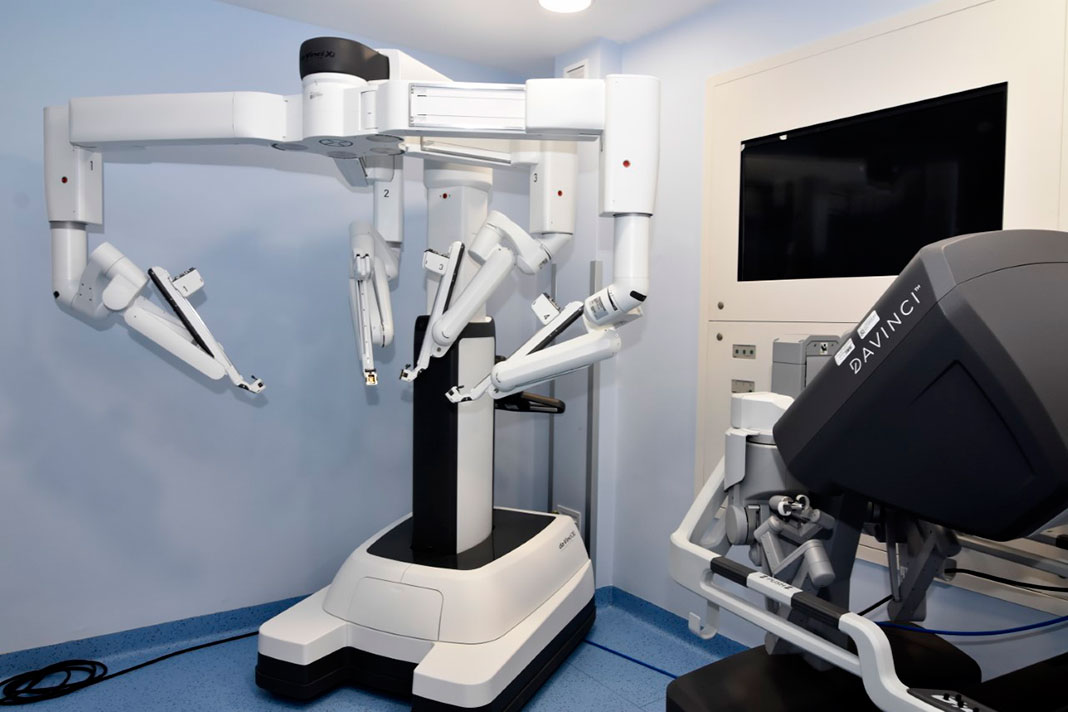
\includegraphics[width=5cm, height=3.5cm]{img/davinci.jpg}
        \label{fig:davinci}
        \end{subfigure}\hfill
            \begin{subfigure}{\textwidth}
                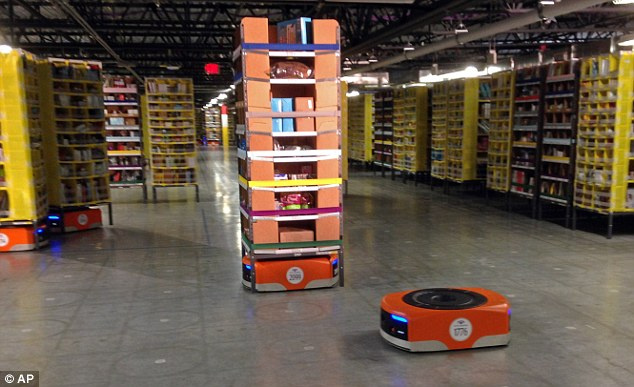
\includegraphics[width=5cm, height=3.5cm]{img/robots-amazon.jpg}
            \label{fig:amazon}
            \end{subfigure}\hfill
            \label{fig:robotica}
            \end{figure}
		\end{frame}
		
	\begin{frame}
		\frametitle{Robótica educativa}
		\begin{itemize}
			\item Lenguajes de programación visual: Scratch!, LEGO, Kodu, Snap! o Blockly.
		           \begin{figure}[H]
                    \centering
                    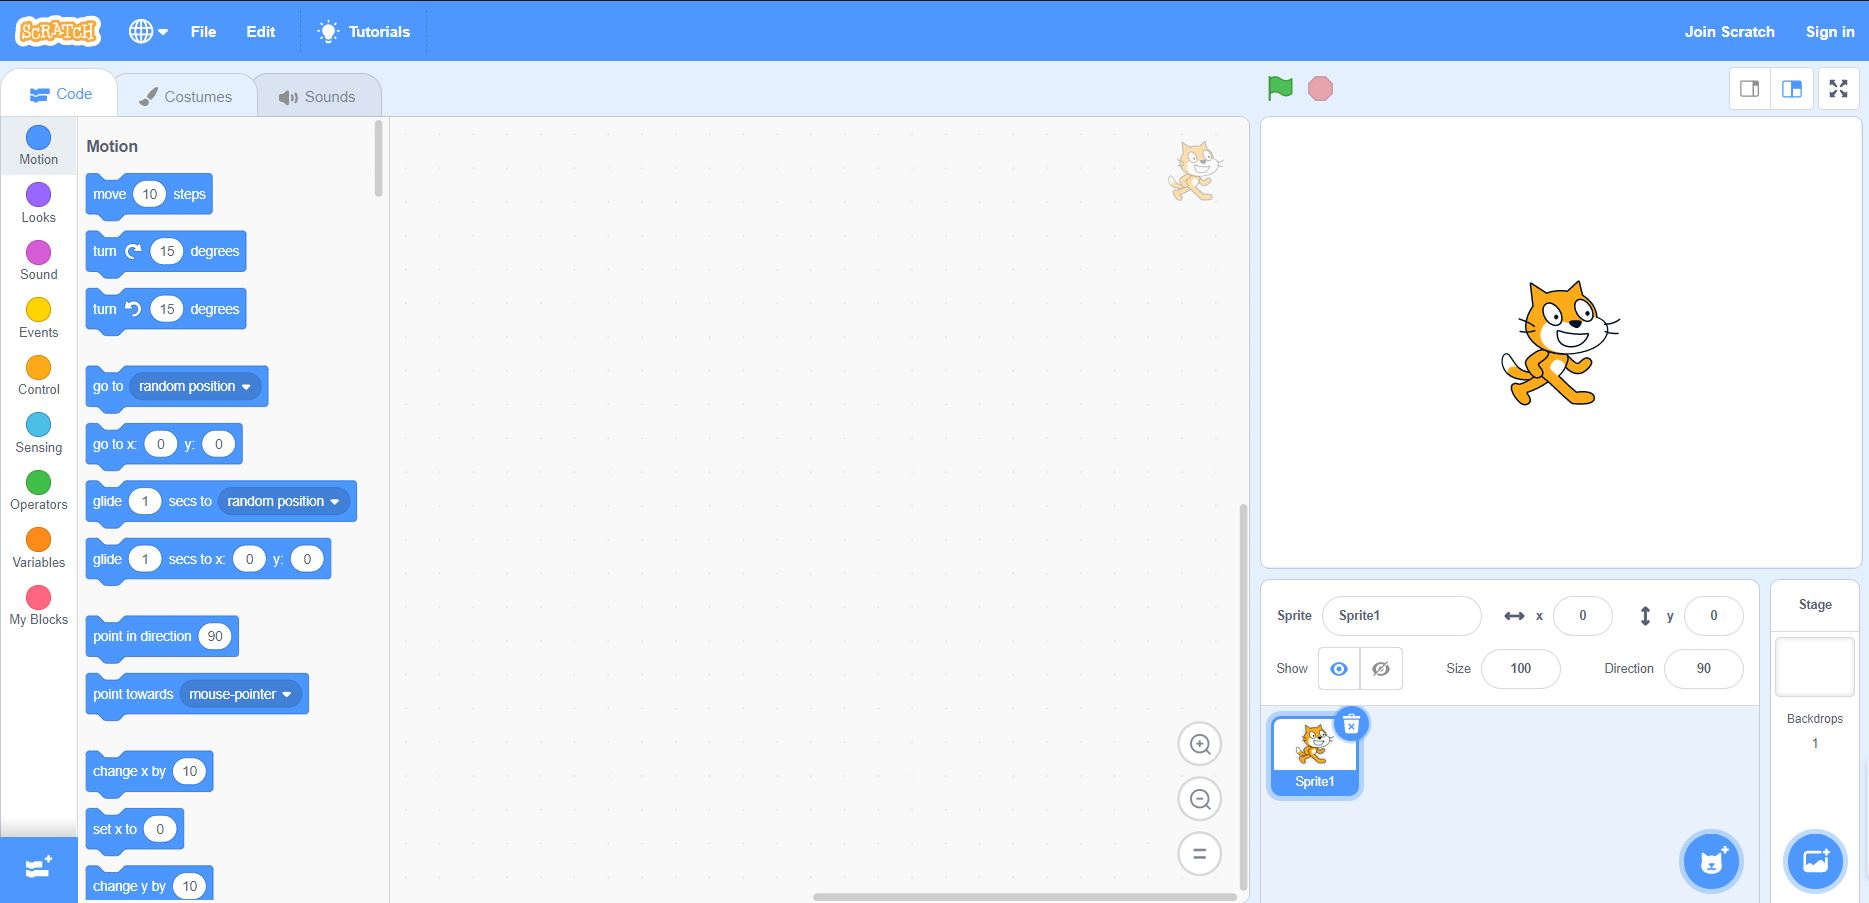
\includegraphics[scale=0.2]{img/scratch.jpg}
                   \label{fig:scratch}
                    \end{figure}
            \item Plataformas hardware: \textit{LEGO mindstorm}, \textit{Makeblock} o \textit{Arduino}.
		\end{itemize}
	\end{frame}

	\section{Herramientas}
		\begin{frame}
			\frametitle{Herramientas}
                \begin{figure}[H]
                \centering
                \begin{subfigure}{\textwidth}
                    
\includegraphics[width=3cm, height=3cm]{img/js.png}
                \label{fig:figure2_4}
                \end{subfigure}
                \begin{subfigure}{\textwidth}
                    
\includegraphics[width=3cm, height=3cm]{img/aframe.png}
                \label{fig:figure2_5}
                \end{subfigure}\hfill
                \begin{subfigure}{\textwidth}
                    
\includegraphics[width=3cm, height=3cm]{img/blockly.png}
                \label{fig:figure2_6}
                \end{subfigure}\hfill
                \begin{subfigure}{\textwidth}
                    
\includegraphics[width=3cm, height=3cm]{img/blender.png}
                \label{fig:figure2_7}
                \end{subfigure}\hfill
                    \begin{subfigure}{\textwidth}
                        
\includegraphics[width=3cm, height=3cm]{img/webpack.jpeg}
                    \label{fig:figure2_9}
                    \end{subfigure}\hfill
                    \begin{subfigure}{\textwidth}
                        
\includegraphics[width=3cm, height=2cm]{img/npm.png}
                    \label{fig:figure2_8}
                    \end{subfigure}\hfill
                    \label{fig:herramientas}
                    \end{figure}
        \end{frame}
        
	\begin{frame}
	\frametitle{WebSim}
	\begin{itemize}
	    \item \textit{WebSim} es un simulador robótico diseñado para enseñar conceptos básicos de tecnología e iniciar a niños en robótica y programación.
	    
	    \item Permite conectar un editor de texto o bloques a un robot simulado. 
	\end{itemize}
\end{frame}
		
	\section{Objetivos}
		\begin{frame}
			\frametitle{Objetivos}
			\begin{enumerate}
				\item Ampliar el simulador robótico WebSim para dar soporte a drones
				\item Teleoperadores para poder manejar los robots sin necesidad de programar.
				\item Nuevos ejercicios individuales- Ficheros de configuración y nuevos modelos.
				\item Nuevos ejercicios competitivos y evaluadores automáticos. 
			\end{enumerate}
		\end{frame}

	\section{Mejoras a WebSim}
		\begin{frame}
			\frametitle{Soporte a drones y otros modelos}
				\begin{itemize}
				\item Drivers
				\item Modelo 3D
				\item Bloques de Scratch
				\item Otros modelos 
			\end{itemize}
		\end{frame}
			\begin{frame}
			\frametitle{Soporte a drones: Drivers}
			\begin{itemize}
				\item \textit{setL}
				\item \textit{getL}
				\item \textit{despegar}
				\item \textit{aterrizar}
				\item \textit{updatePosition}
			\end{itemize}
		\end{frame}
% 			\begin{frame}
% 			\frametitle{Soporte a drones: Drivers}
% 			\begin{itemize}
% 				\item Sistema de físicas
% 			\end{itemize}
% 		\end{frame}
				
    	\begin{frame}
			\frametitle{Soporte a drones: Modelo 3D}
            \begin{itemize}
                \item Rotación del modelo para seguir el mismo sistema de coordenadas que \textit{A-Frame}.
                \item Modificación de luz y texturas. \item Animación de las helices. 
            \end{itemize}
    	\end{frame}
    	
    	\begin{frame}
			\frametitle{Soporte a drones: Modelo 3D}
           \begin{figure}[H]
            \centering
            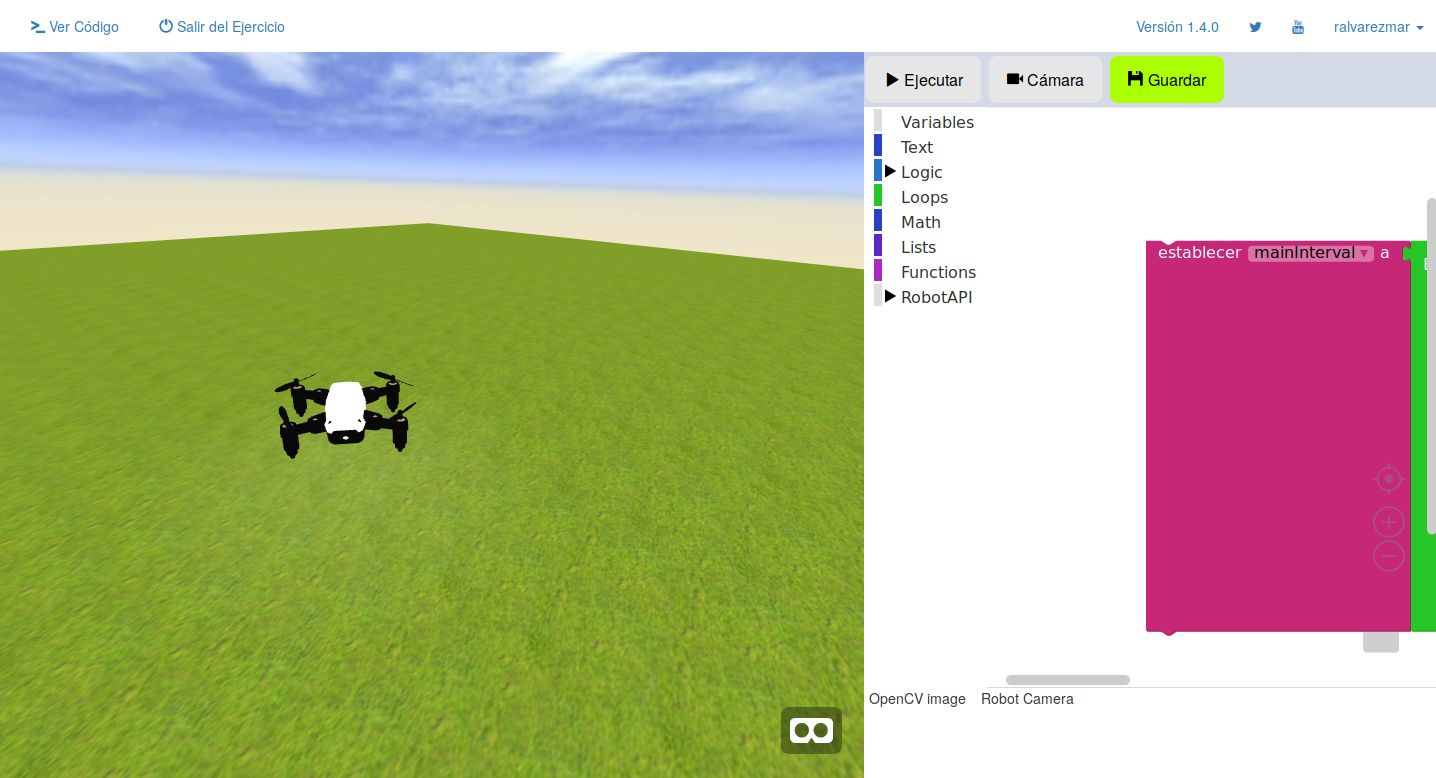
\includegraphics[scale=0.2]{img/WebsimDrone.png}
           \label{fig:escenarioDrone}
            \end{figure}
    	\end{frame}
    	
    	   \begin{frame}
			\frametitle{Soporte a drones: Modelo 3D}
          \begin{figure}[H]
        \centering
        \begin{subfigure}{\textwidth}
         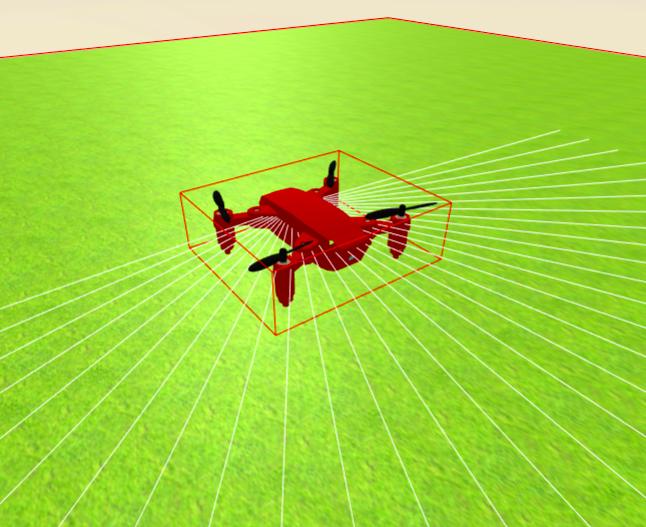
\includegraphics[width=4cm, height=3cm]{img/red_drone.png}
 \label{fig:drone_rojo}
        \end{subfigure}
        \begin{subfigure}{\textwidth}
         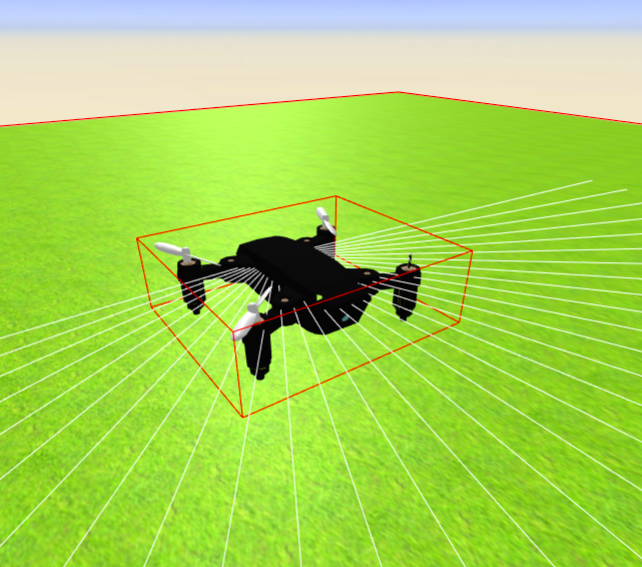
\includegraphics[width=4cm, height=3cm]{img/black_drone.png}
   \label{fig:drone_negro}
        \end{subfigure}
        \begin{subfigure}{\textwidth}
         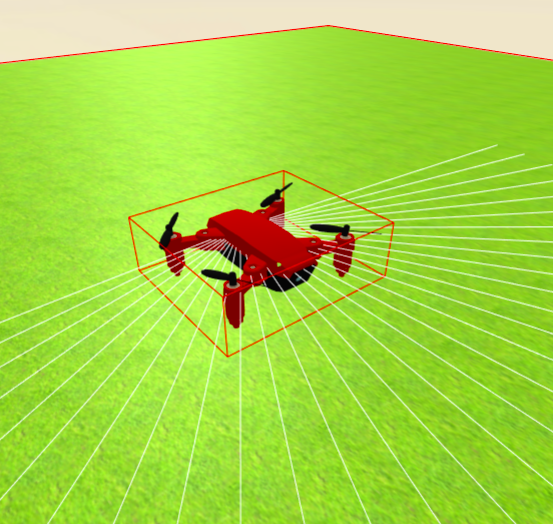
\includegraphics[width=4cm, height=3cm]{img/red_blackdrone.png}
   \label{fig:drone_negrorojo}
        \end{subfigure}
    \end{figure}
    	\end{frame}
		   
		\begin{frame}
		\frametitle{Soporte a drones: Bloques Scratch}
		       \begin{figure}[H]
            \centering
            
\includegraphics[scale=0.5]{img/ascensionBlockly.png}
           \label{fig:ascension}
            \end{figure}
                 \begin{figure}[H]
            \centering
            
\includegraphics[scale=0.5]{img/verticalBlockly.png}
           \label{fig:vertica}
            \end{figure}
            \begin{figure}[H]
            \centering
            
\includegraphics[scale=0.5]{img/aterrizarBlockly.png}
           \label{fig:vertica}
            \end{figure}
               \begin{figure}[H]
            \centering
            
\includegraphics[scale=0.5]{img/despegarBlockly.png}
           \label{fig:vertica}
            \end{figure}
		\end{frame}
		
		
		
		\begin{frame}
			\frametitle{Otros modelos}
		\begin{figure}[H]
        \centering
        \begin{subfigure}{\textwidth}
         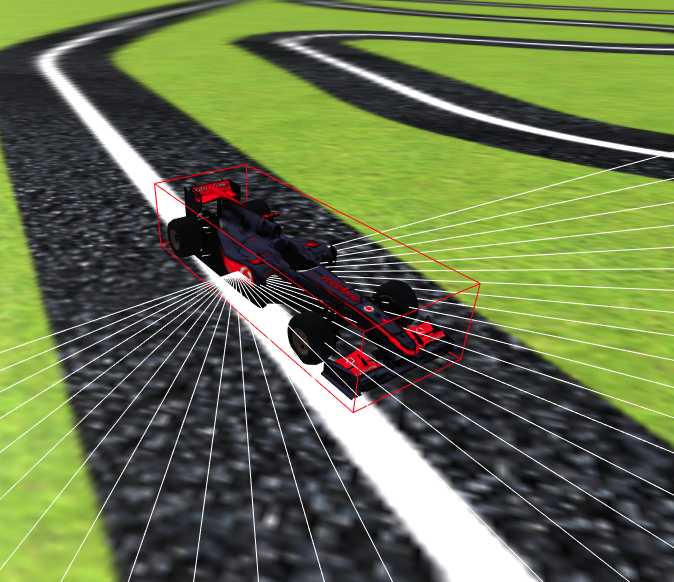
\includegraphics[width=4cm, height=3cm]{img/f1_williams.png}
 \label{fig:f1williams}
        \end{subfigure}
        \begin{subfigure}{\textwidth}
         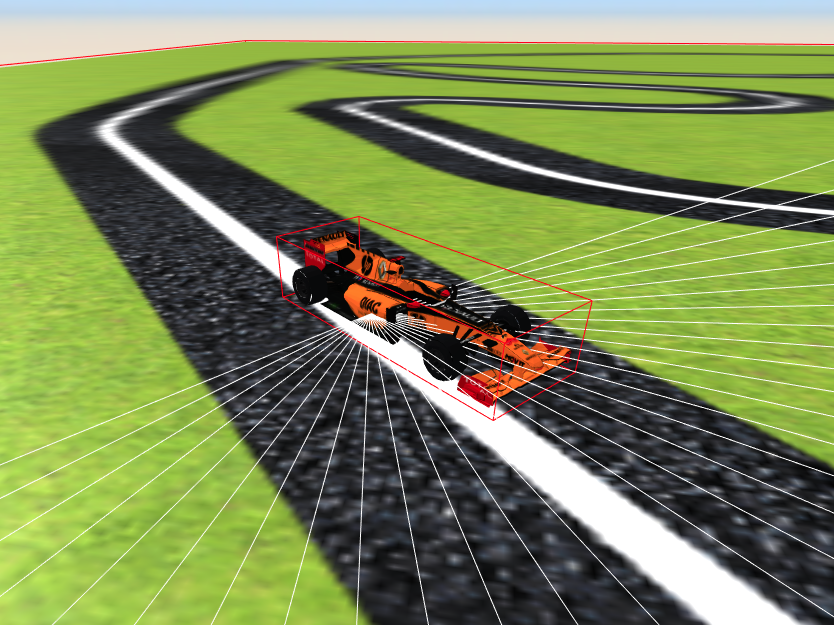
\includegraphics[width=4cm, height=3cm]{img/f1_renault.png}
   \label{fig:f1renault}
        \end{subfigure}
        \begin{subfigure}{\textwidth}
         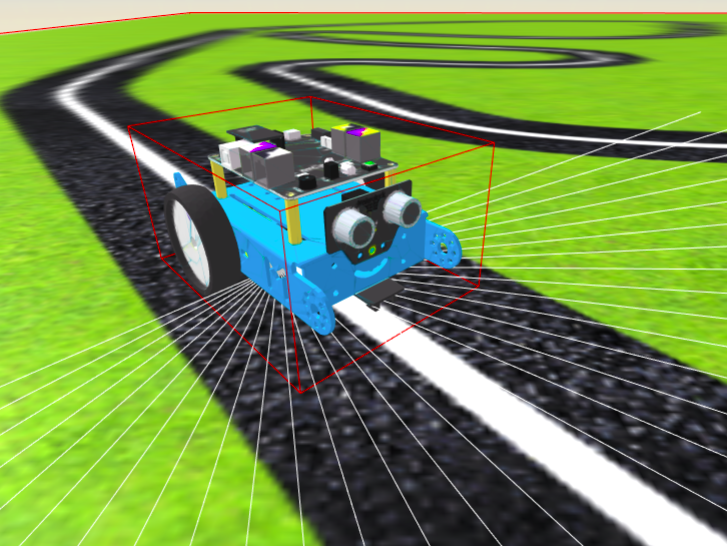
\includegraphics[width=4cm, height=3cm]{img/mBot_model.png}
   \label{fig:mbot}
        \end{subfigure}
        \end{figure}
		\end{frame}
		
		\begin{frame}
		\frametitle{Teleoperadores}
    		\begin{itemize}
    			\item Posibilidad de controlar los robots sin necesidad de programarlos
		    \end{itemize}
    		\begin{figure}{\textwidth}
    		\centering
             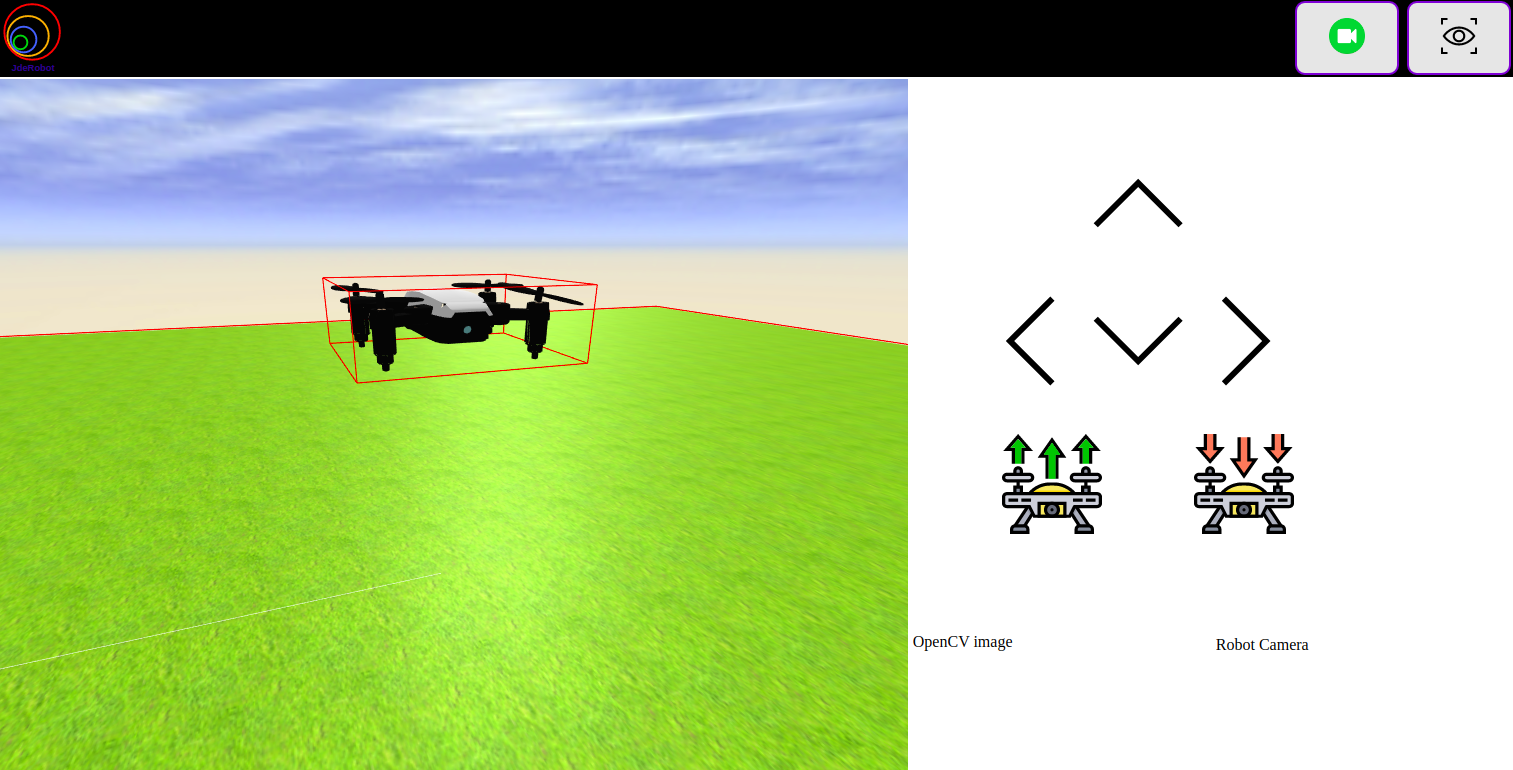
\includegraphics[scale=0.18]{img/drone_teleoperator.png}
             \label{fig:teleopdrone}
            \end{figure}
		\end{frame}
		
		
		\begin{frame}
		\frametitle{Teleoperadores: Arquitectura}
             \begin{wrapfigure}{L}{0.5\textwidth}
            \centering
            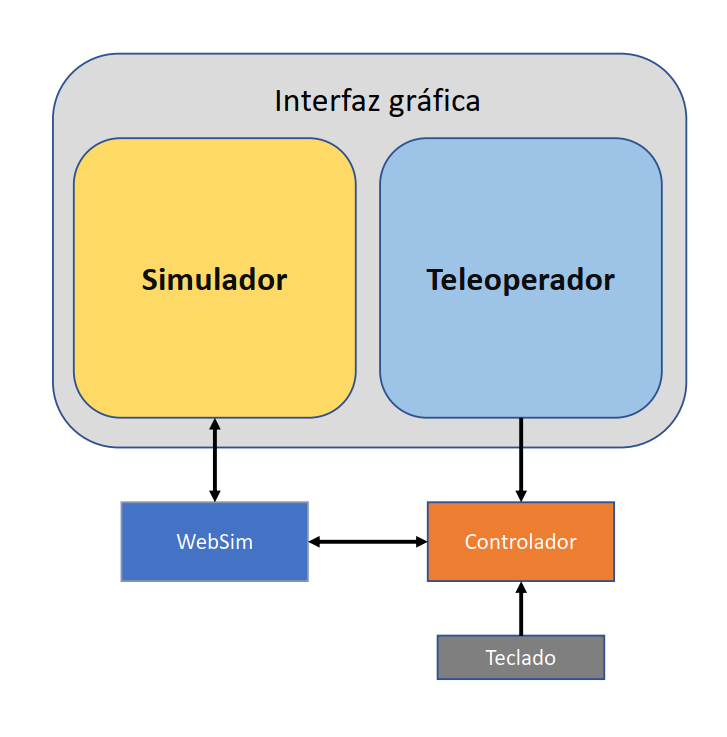
\includegraphics[width=0.5\textwidth]{img/arquitecturaTeleoperador.png}
            \label{fig:droneteleop}
            \end{wrapfigure}
              \item Se envía un evento cuando se pulsa uno de los botones de la interfaz gráfica o del teclado.
              \item Mediante un controlador se obtienen las velocidades del robot y se envían las nuevas.
              \item  \textit{WebSim} representa las nuevas velocidades comandadas en el simulador web.
		\end{frame}
		
		\begin{frame}
			\frametitle{Teleoperadores: configuración}
			\newline
		    \begin{itemize}
		        \item Ficheros de configuración creados para crear el escenario sin necesidad de tener los elementos en el código fuente.
		        \item Formato JSON en el que se especifica escenario simulado, robot elegido, distintos parámetros como la gravedad, etc. 
		    \end{itemize}
		\end{frame}
		
			\begin{frame}
			\frametitle{Teleoperadores: configuración}
		\begin{figure}{\textwidth}
    		\centering
             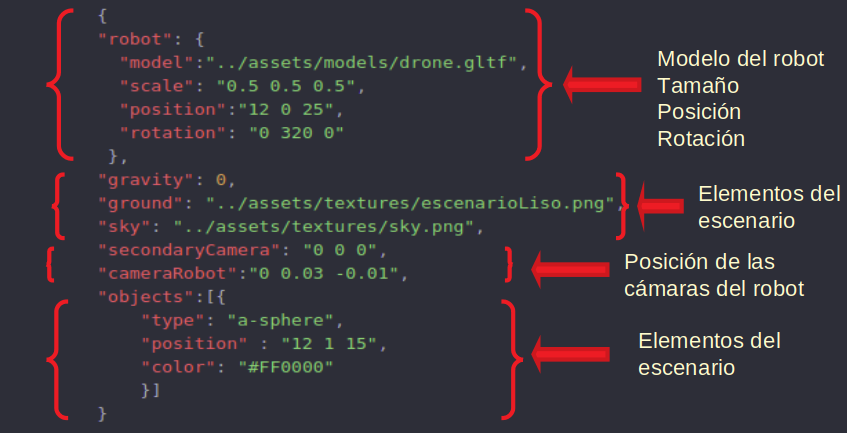
\includegraphics[scale=0.35]{img/configuracion.png}
             \label{fig:configuracion}
            \end{figure}
		\end{frame}
		
		\section{Ejercicios individuales}
		\begin{frame}
			\frametitle{Sigue líneas}
        		\begin{figure}[H]
                \centering
                \begin{subfigure}{\textwidth}
                 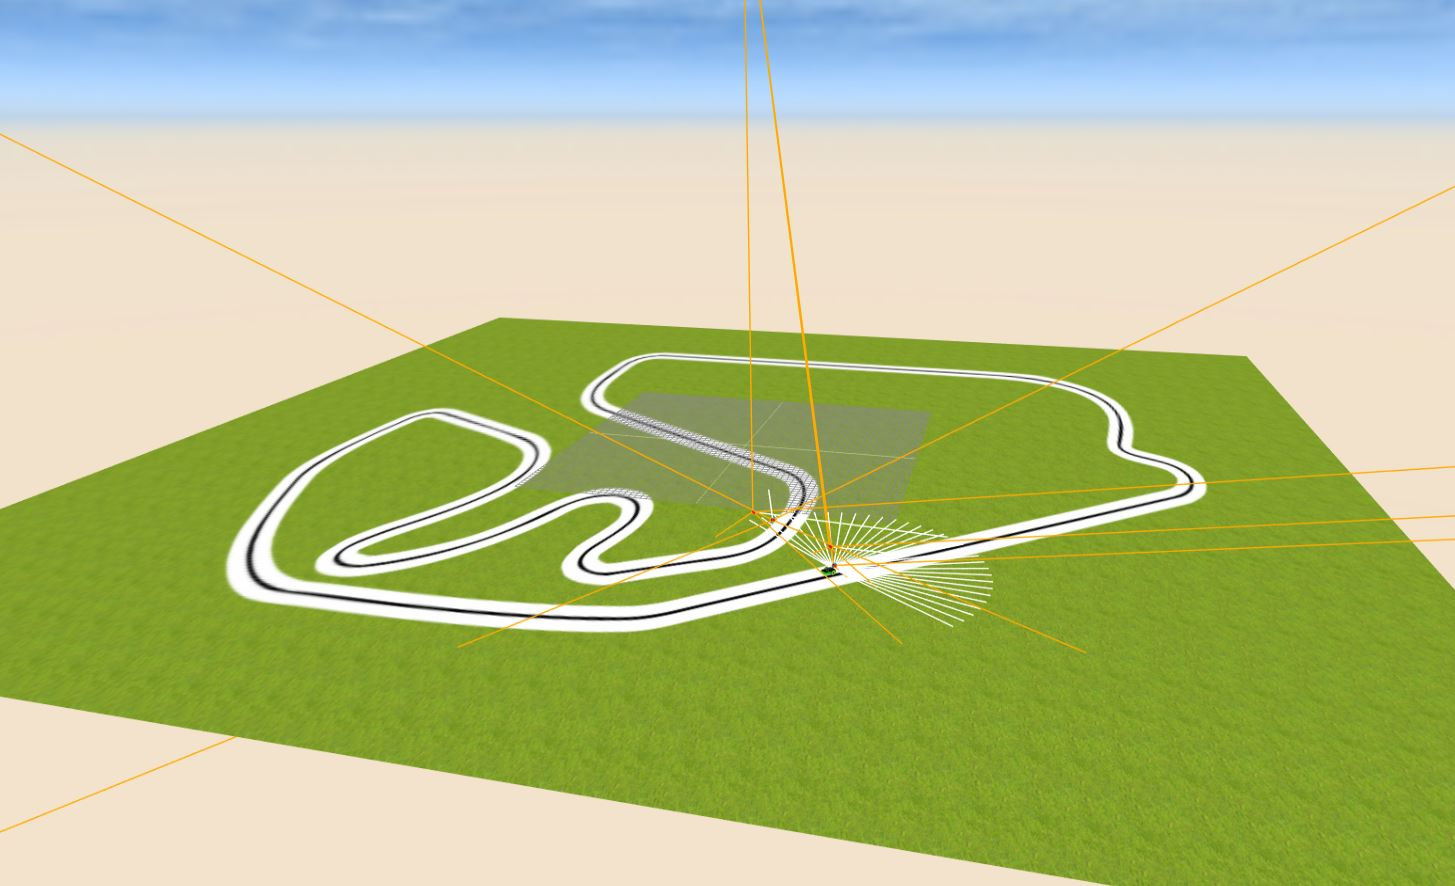
\includegraphics[scale=0.15]{img/siguelineas_ir.JPG}
                 \label{fig:ir}
                \end{subfigure}
                \begin{subfigure}{\textwidth}
                 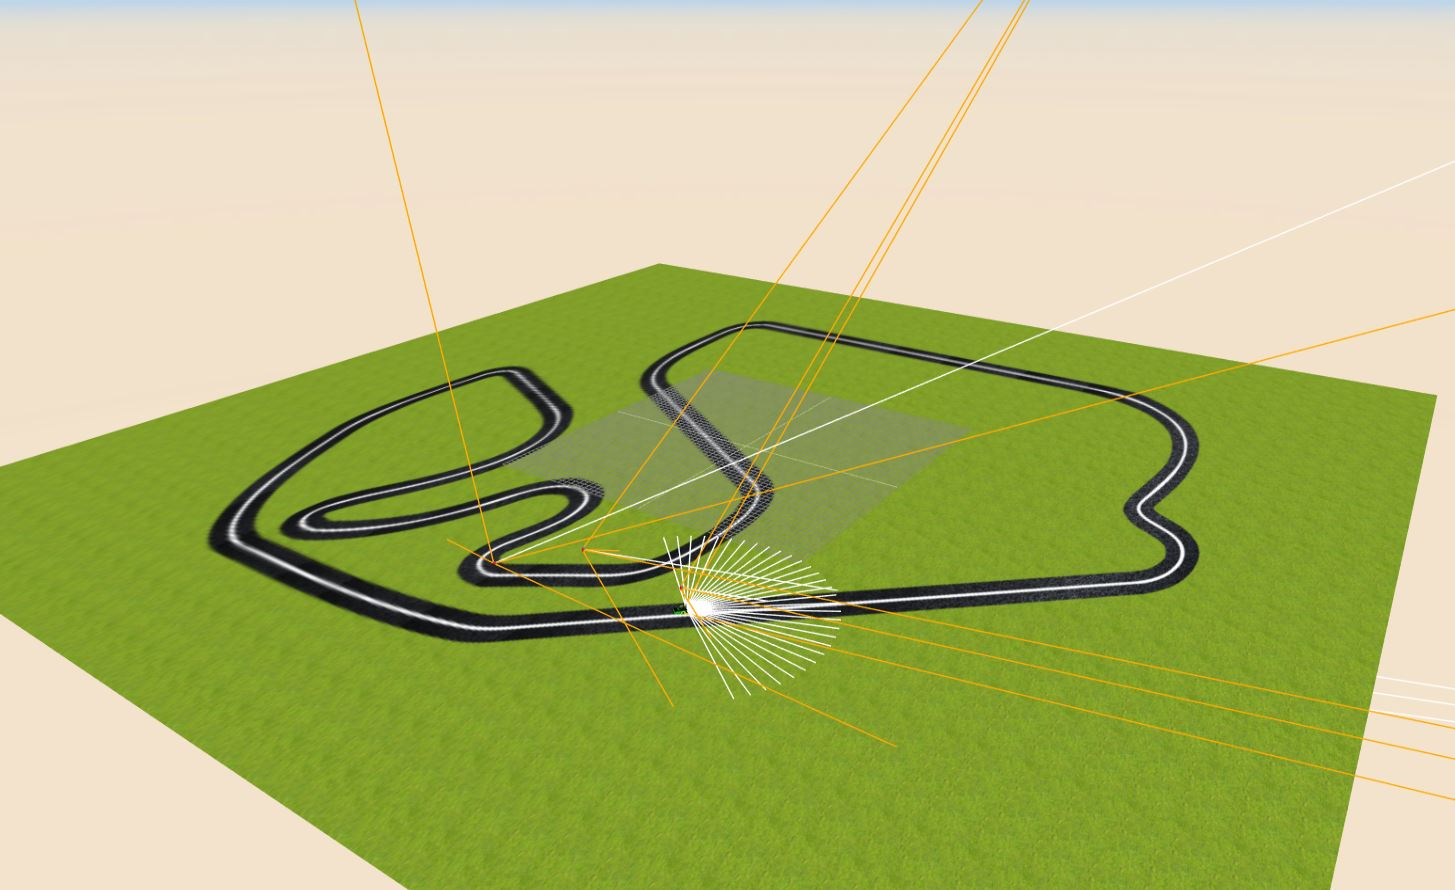
\includegraphics[scale=0.15]{img/pibot_vision.JPG}
                \label{fig:vision}
                \end{subfigure}
                \end{figure}
        \end{frame}
		
		
		\begin{frame}
			\frametitle{Choca-gira}
						\begin{figure}{\textwidth}
             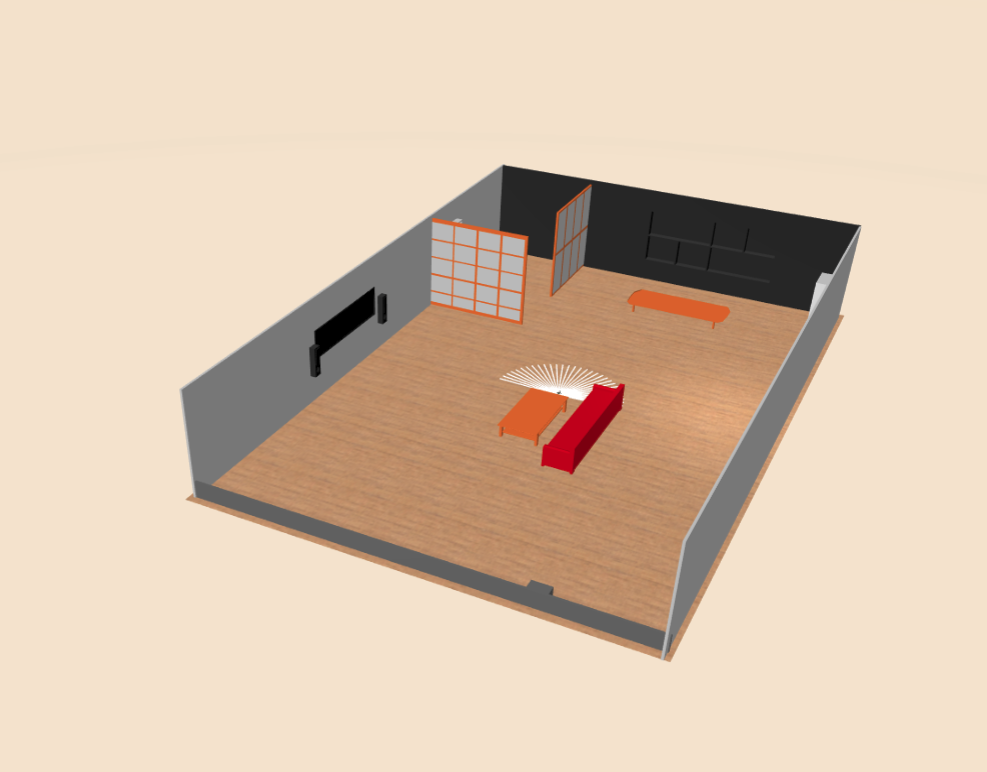
\includegraphics[scale=0.25]{img/bump&go.png}
             \label{fig:chocagira}
            \end{figure}
		\end{frame}
		
		\begin{frame}
			\frametitle{Sigue pelota}
			\begin{subfigure}{\textwidth}
              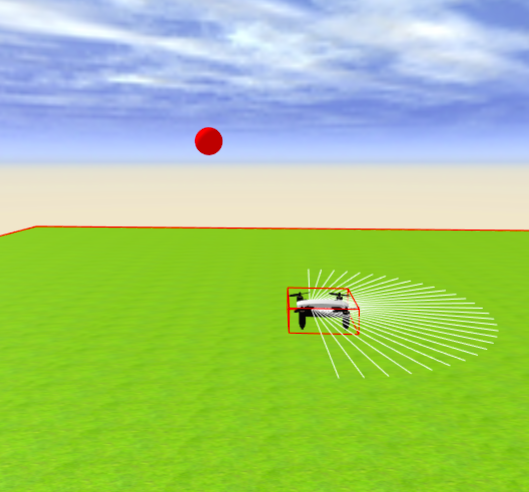
\includegraphics[width=3cm, height=3cm]{img/followBallTello2.png}
            \label{fig:figure2_2}
            \end{subfigure}\hfill
            \begin{subfigure}{\textwidth}
                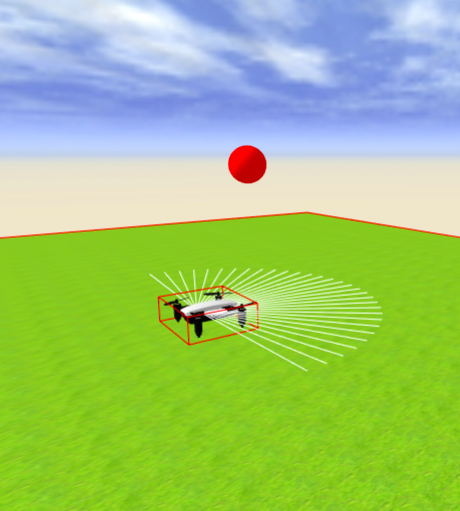
\includegraphics[width=3cm, height=3cm]{img/followBallTello3.png}
            \label{fig:figure2_3}
            \end{subfigure}\hfill
            \begin{subfigure}{\textwidth}
                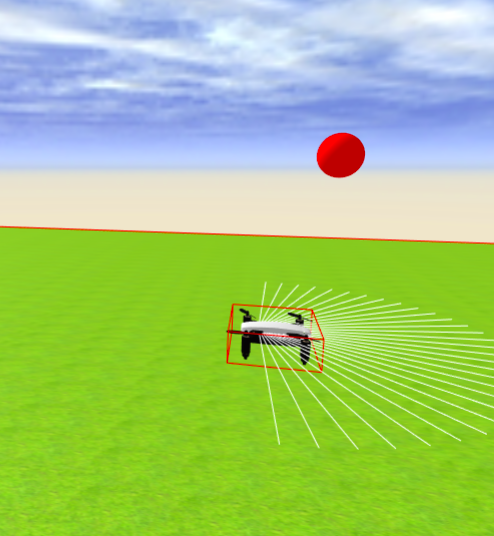
\includegraphics[width=3cm, height=3cm]{img/followBallTello4.png}
            \label{fig:figure2_4}
            \end{subfigure}
            \begin{subfigure}{\textwidth}
                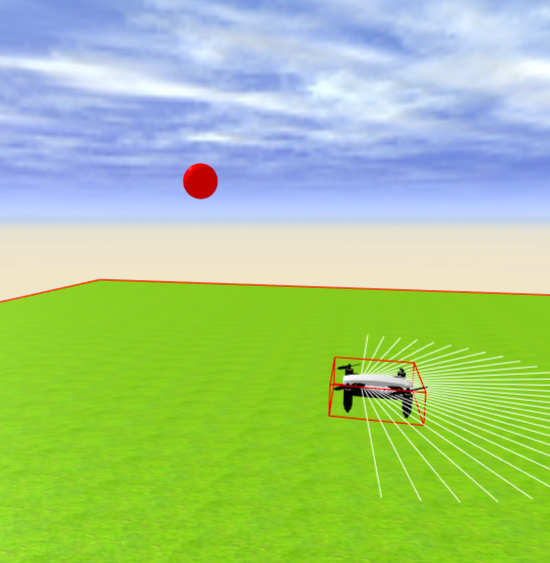
\includegraphics[width=3cm, height=3cm]{img/followBallTello6.png}
            \label{fig:figure2_6}
            \end{subfigure}\hfill
            \begin{subfigure}{\textwidth}
                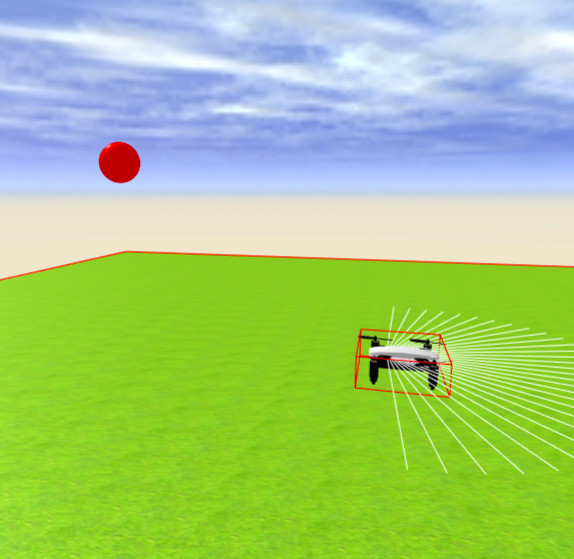
\includegraphics[width=3cm, height=3cm]{img/followBallTello7.png}
            \label{fig:figure2_7}
            \end{subfigure}\hfill
            \begin{subfigure}{\textwidth}
                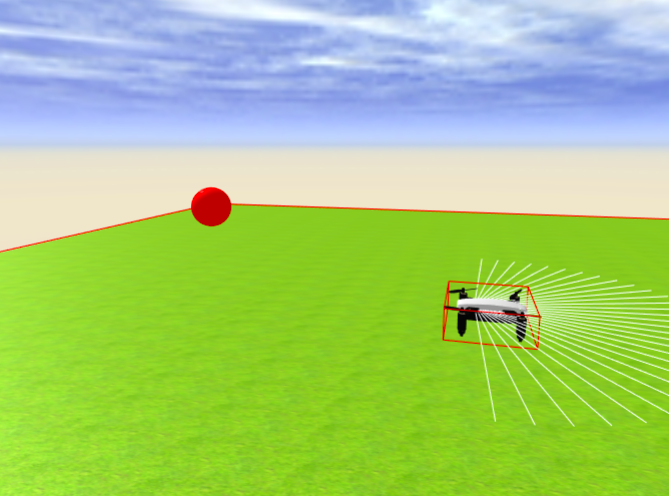
\includegraphics[width=3cm, height=3cm]{img/followBallTello8.png}
            \label{fig:figure2_8}
            \end{subfigure}
		\end{frame}
		
		
		\begin{frame}
			\frametitle{Cuadrado-drone}
					\begin{figure}{\textwidth}
    		\centering
             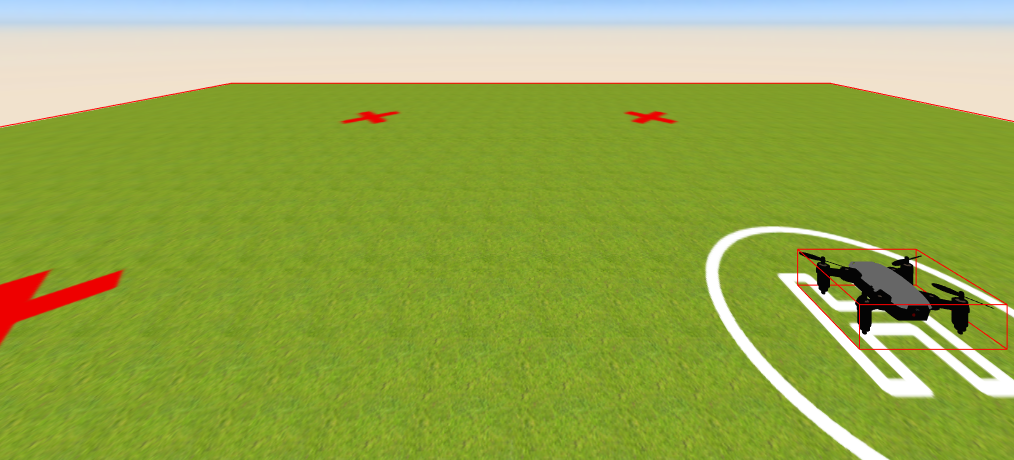
\includegraphics[scale=0.4]{img/cuadradoDrone.png}
             \label{fig:configuracion}
            \end{figure}
		\end{frame}
		\begin{frame}
			\frametitle{Atraviesa bosque}
       \begin{figure}
         \href{https://youtu.be/z3n47wWHDFc}
              {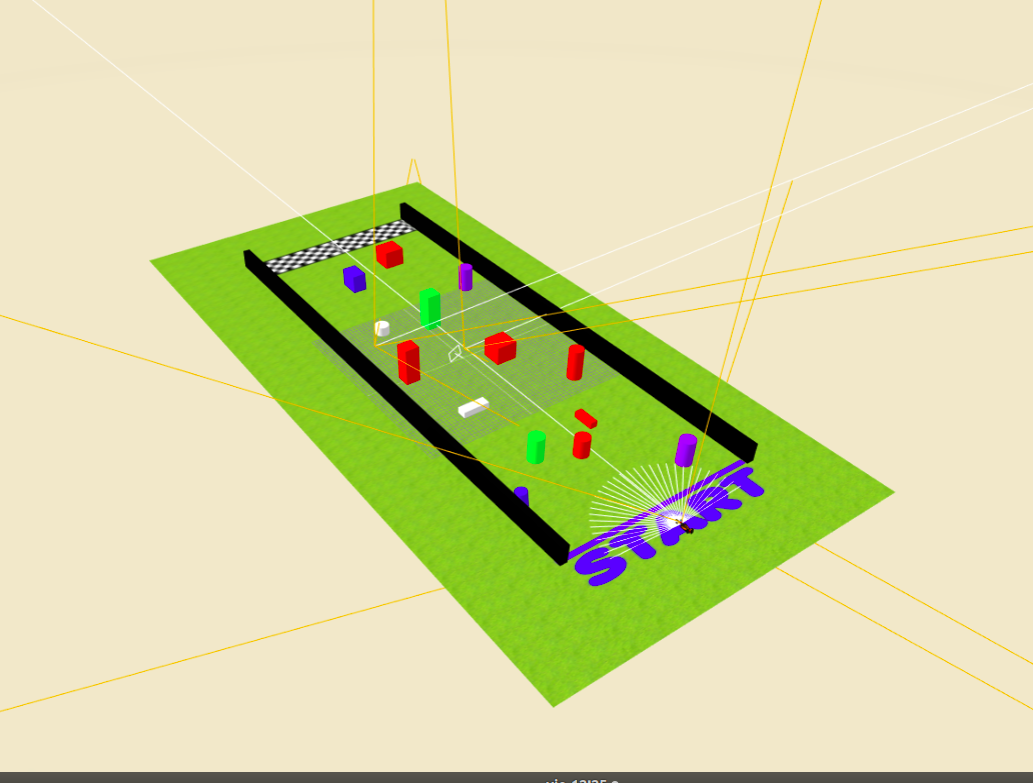
\includegraphics[width=0.8\textwidth]{img/atraviesabosque-indiv.png}}
       \end{figure}

		\end{frame}
		\section{Ejercicios competitivos}
		\begin{frame}
			\frametitle{Arquitectura de cómputo}
			\begin{itemize}
			    \item Módulo \textit{brains} ampliado:
			    \begin{itemize}\itemsep5pt
			        \item Módulo \textit{evaluators}. Lanza un hilo que tiene acceso a los sensores de los \textit{robots} y evalúa la calidad de su comportamiento.
			        \item  Módulo \textit{agents}. Ejecuta el código en un robot de un fichero creado previamente. 
			    \end{itemize}
			\end{itemize}
		\end{frame}
		
		\begin{frame}
			\frametitle{Arquitectura de cómputo}
			\begin{itemize}
			     \item Nuevos editores para ejercicios competitivos:
			\end{itemize}
				\begin{figure}[H]
                \centering
                \begin{subfigure}{\textwidth}
                 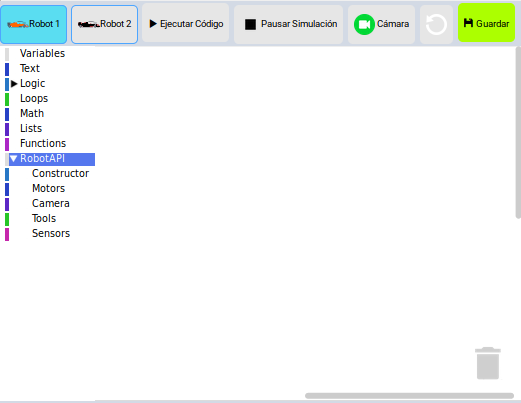
\includegraphics[width=5cm, height=3.5cm]{img/competitivoEditorScratch.png}
                 \label{fig:ir}
                \end{subfigure}
                \begin{subfigure}{\textwidth}
                 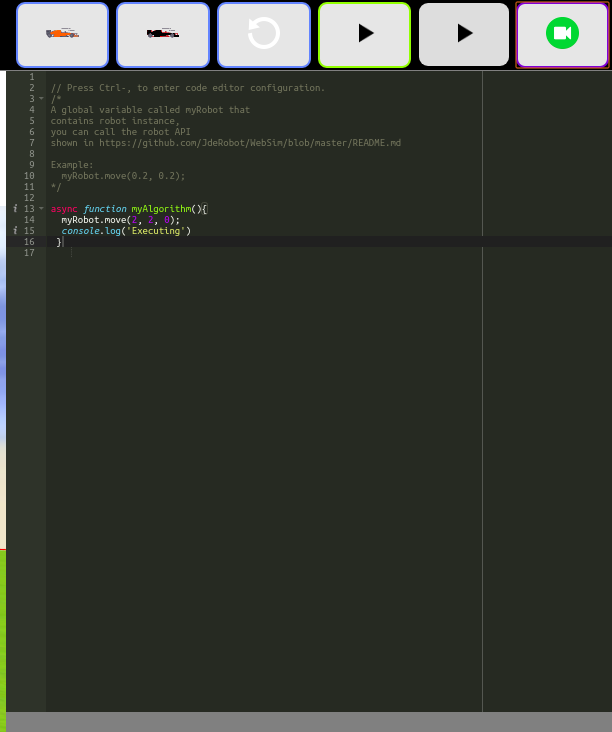
\includegraphics[width=4cm, height=3.5cm]{img/competitiveEditorJavascript.png}
                \label{fig:vision}
                \end{subfigure}
                \end{figure}
		\end{frame}
		
		\begin{frame}
			\frametitle{Atraviesa bosque competitivo}
						\begin{figure}{\textwidth}
             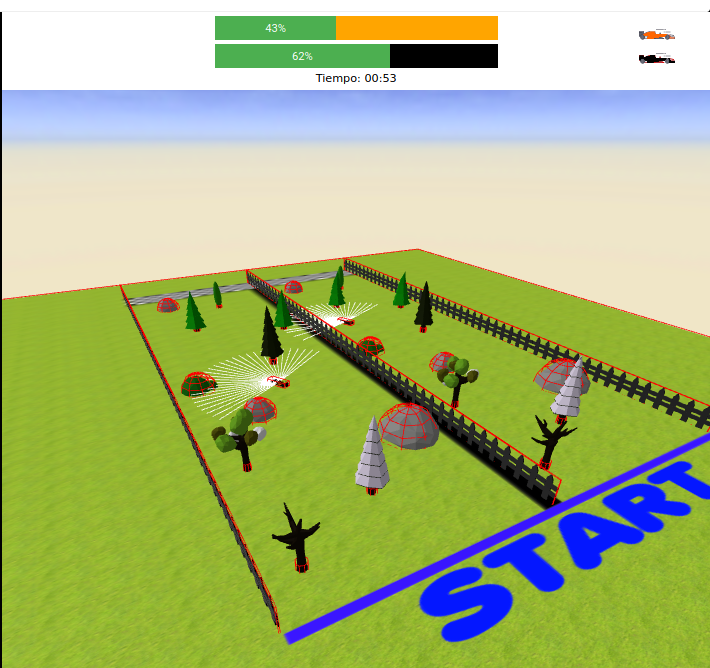
\includegraphics[scale=0.25]{img/evaluador_forest.png}
             \label{fig:configuracion}
            \end{figure}
		\end{frame}
		
		\begin{frame}
			\frametitle{Siguelíneas visión competitivo}
       \begin{figure}
         \href{https://youtu.be/OaA7_wsXhk8}
              {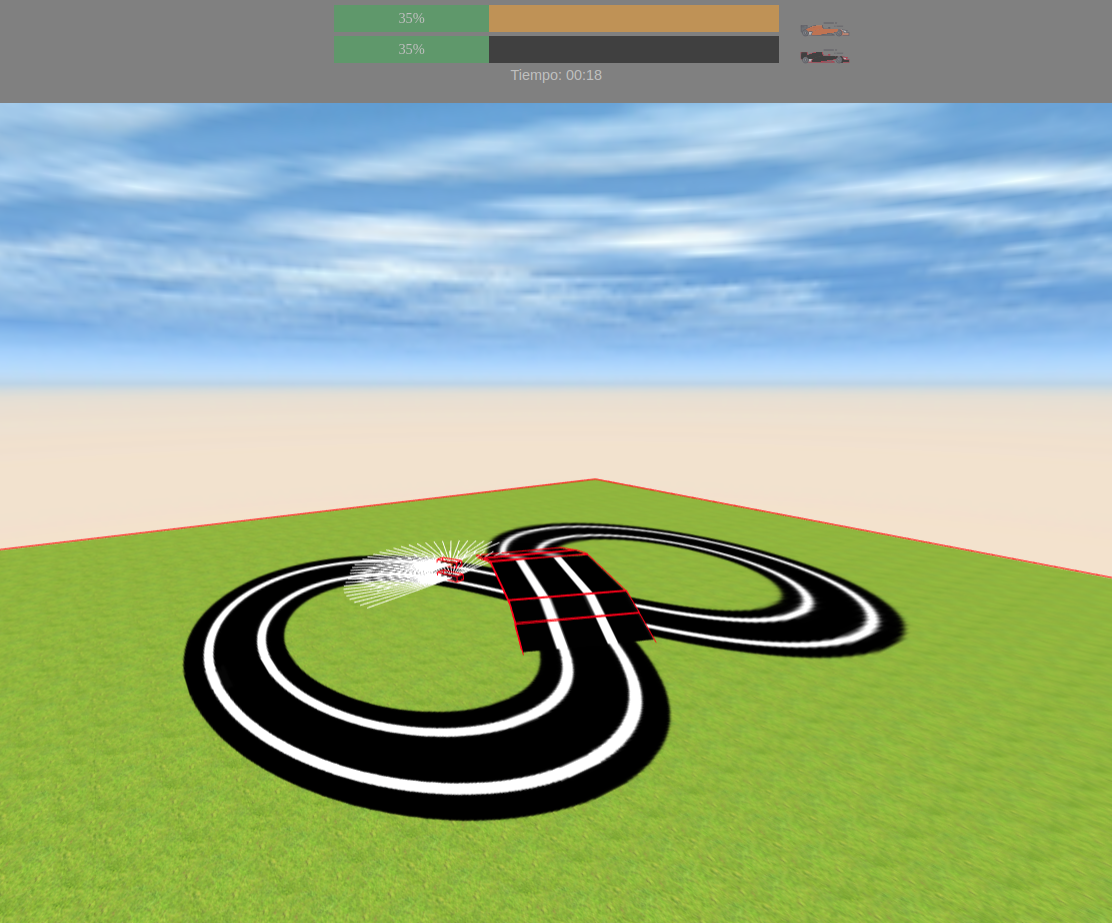
\includegraphics[width=0.8\textwidth]{img/evaluator_follow_line.png}}
       \end{figure}
		\end{frame}
		

		\begin{frame}
			\frametitle{Gato-ratón}
       \begin{figure}
         \href{https://youtu.be/xA9Emhdk_HQ}
              {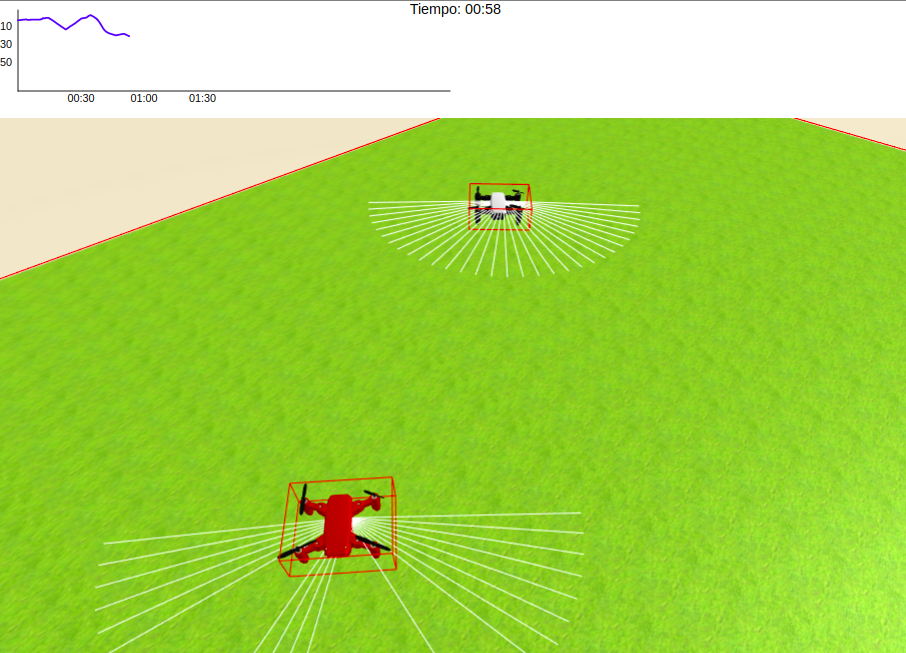
\includegraphics[width=0.8\textwidth]{img/evaluador_drone.png}}
       \end{figure}
		\end{frame}

	\section{Conclusiones}
		\begin{frame}
			\frametitle{Conclusiones}
			\begin{itemize}
				\item Soporte a \textit{drones} para \textit{WebSim}. 
				\item Nuevos ejercicios que aprovechan las funcionalidades existentes de \textit{WebSim}.
				\item Nuevos ejercicios competitivos que implementan nueva funcionalidad como los evaluadores automáticos. 
			\end{itemize}
		\end{frame}
	
	\appendix

	\backupbegin
	
	\backupend

\end{document}